% Options for packages loaded elsewhere
\PassOptionsToPackage{unicode}{hyperref}
\PassOptionsToPackage{hyphens}{url}
%
\documentclass[
]{article}
\usepackage{lmodern}
\usepackage{amssymb,amsmath}
\usepackage{ifxetex,ifluatex}
\ifnum 0\ifxetex 1\fi\ifluatex 1\fi=0 % if pdftex
  \usepackage[T1]{fontenc}
  \usepackage[utf8]{inputenc}
  \usepackage{textcomp} % provide euro and other symbols
\else % if luatex or xetex
  \usepackage{unicode-math}
  \defaultfontfeatures{Scale=MatchLowercase}
  \defaultfontfeatures[\rmfamily]{Ligatures=TeX,Scale=1}
\fi
% Use upquote if available, for straight quotes in verbatim environments
\IfFileExists{upquote.sty}{\usepackage{upquote}}{}
\IfFileExists{microtype.sty}{% use microtype if available
  \usepackage[]{microtype}
  \UseMicrotypeSet[protrusion]{basicmath} % disable protrusion for tt fonts
}{}
\makeatletter
\@ifundefined{KOMAClassName}{% if non-KOMA class
  \IfFileExists{parskip.sty}{%
    \usepackage{parskip}
  }{% else
    \setlength{\parindent}{0pt}
    \setlength{\parskip}{6pt plus 2pt minus 1pt}}
}{% if KOMA class
  \KOMAoptions{parskip=half}}
\makeatother
\usepackage{xcolor}
\IfFileExists{xurl.sty}{\usepackage{xurl}}{} % add URL line breaks if available
\IfFileExists{bookmark.sty}{\usepackage{bookmark}}{\usepackage{hyperref}}
\hypersetup{
  hidelinks,
  pdfcreator={LaTeX via pandoc}}
\urlstyle{same} % disable monospaced font for URLs
\usepackage{longtable,booktabs}
% Correct order of tables after \paragraph or \subparagraph
\usepackage{etoolbox}
\makeatletter
\patchcmd\longtable{\par}{\if@noskipsec\mbox{}\fi\par}{}{}
\makeatother
% Allow footnotes in longtable head/foot
\IfFileExists{footnotehyper.sty}{\usepackage{footnotehyper}}{\usepackage{footnote}}
\makesavenoteenv{longtable}
\usepackage{graphicx}
\makeatletter
\def\maxwidth{\ifdim\Gin@nat@width>\linewidth\linewidth\else\Gin@nat@width\fi}
\def\maxheight{\ifdim\Gin@nat@height>\textheight\textheight\else\Gin@nat@height\fi}
\makeatother
% Scale images if necessary, so that they will not overflow the page
% margins by default, and it is still possible to overwrite the defaults
% using explicit options in \includegraphics[width, height, ...]{}
\setkeys{Gin}{width=\maxwidth,height=\maxheight,keepaspectratio}
% Set default figure placement to htbp
\makeatletter
\def\fps@figure{htbp}
\makeatother
\setlength{\emergencystretch}{3em} % prevent overfull lines
\providecommand{\tightlist}{%
  \setlength{\itemsep}{0pt}\setlength{\parskip}{0pt}}
\setcounter{secnumdepth}{-\maxdimen} % remove section numbering

\author{}
\date{}

\begin{document}

\hypertarget{modelsim}{%
\section{ModelSim}\label{modelsim}}

ModelSim is a full-featured VHDL simulator. With VHDL, you can create
logic designs consisting of any size. To verify functional operation you
need to simulate your design to see whether it works like expected.
Therefore, test benches are used. They contain so-called stimuli or test
vectors, simply said: values for the input signals. These values are
applied to the input signals and then the corresponding output signals
are compared with the expected values.

To simulate a specific design one has to provide two kinds of files to
the ModelSim simulator: VHDL files that contain your processor design
and a testbench file that creates the needed environment. ASIP Meister
creates the VHDL files for your processor design automatically and the
designer does not have to take care about the VHDL implementation of the
processor. We provide the testbench and you can find it in the
\emph{TEM­PLATE\_­PRO­JECT/ModelSim} directory (directory structure is
explained in Chapter~2.2.2). This testbench generates a reset and a
clock signal to the CPU. Furthermore, it contains simulated data- and
instruction-memory for the CPU. These simulated memories have to be
initialized with memory images that are read from \emph{TestData.DM} and
\emph{TestData.IM}, before the CPU can start executing the application.
The \emph{Makefile} script creates these memory images automatically
during ``\emph{make sim}'' or ``\emph{make dlxsim}'' and are copied to
the \emph{ModelSim} directory of your current ASIP Meister project (so
you are always simulating the last application that was compiled). After
the simulation of the application is finished, you will find a memory
image of the final data memory \emph{TestData.OUT} that contains the
results of the application if they are stored in data memory.

\hypertarget{tutorial}{%
\subsection{Tutorial}\label{tutorial}}

\hypertarget{create-a-new-modelsim-project}{%
\subsubsection{Create a new ModelSim
Project}\label{create-a-new-modelsim-project}}

Please be aware that it is important that you start ModelSim in the
\emph{ModelSim} directory of your ASIP Meister project, as shown in
Chapter~2.2.2.

On the shell change to the \emph{ModelSim} directory of your project and
invoke ``\emph{vsim \&}''. If ModelSim asks for ``\emph{modelsim.ini}''
choose the default one like
``\emph{/Software/ModelSim/ModelSim\_6.6d/modeltech/modelsim.ini}''

Menu: File \textgreater{} New \textgreater{} Project

Enter a project name e.g. \emph{dlx\_basis1} and change the project
location to the \emph{ModelSim} directory in your project directory.
Confirm the dialog with the OK button.

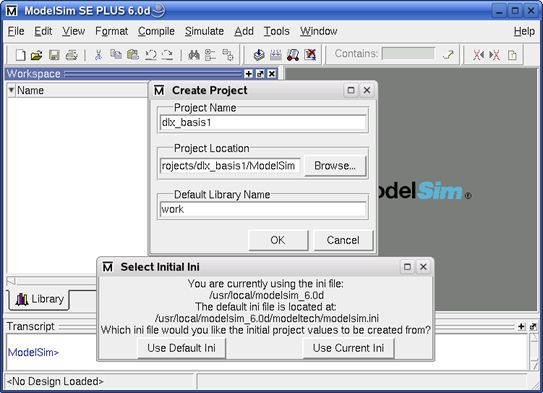
\includegraphics[width=5.65694in,height=4.08958in]{5-1.png}

Figure 5‑1: Creating a ModelSim Project

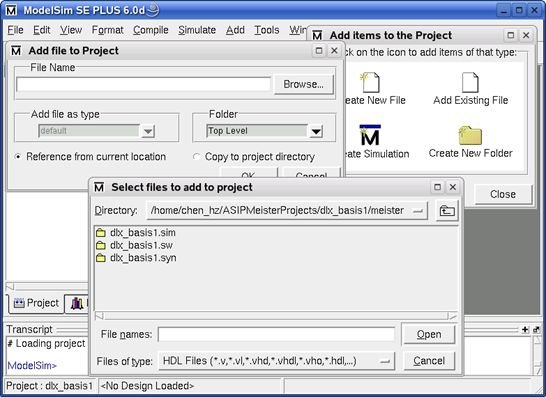
\includegraphics[width=5.68681in,height=4.13403in]{5-2.png}

Figure 5‑2\protect\hypertarget{Fig52}{}{}: Adding Files to a ModelSim
Project

\hypertarget{adding-the-testbench-and-asip-meister-cpu-files}{%
\subsubsection{Adding the Testbench and ASIP Meister CPU
files}\label{adding-the-testbench-and-asip-meister-cpu-files}}

Choose the icon ``\emph{Add Existing File''}. Browse to the VHDL netlist
files for the processor e.g. ``\emph{meister/ dlx\_basis1.syn}''
directory of your ASIP Meister project. Here you will find the VHDL
files for synthesis. There is also a VHDL model of the processor in the
\emph{.sim} directory, but do {not} use the files of the \emph{.sim}
directory, as they do not work properly. Select all the files and
confirm the dialog with ``\emph{open}''. Once again, choose the icon
``\emph{Add Existing File''} to add the testbench files:
\emph{tb\_browstd32.vhd}, \emph{MemoryMapperTypes.vhd},
\emph{MemoryMapper.vhd}, and \emph{Helper.vhd} from the \emph{ModelSim}
directory of your current project.

\hypertarget{compile-the-project}{%
\subsubsection{Compile the project}\label{compile-the-project}}

Menu: Compile \textgreater{} Compile Order \textgreater{} Auto Generate

Every file is compiled and you can see the result of the compile
process. ModelSim determines automatically the compile order of the VHDL
files. After closing the dialog every file should have a green mark
before its name, showing that the compilation was successful (instead of
the question marks), shown in \protect\hyperlink{Fig54}{Figure 5-4}. A
green mark with a yellow dot is a warning that usually indicates a
problem. So take care about the warnings.

\textbf{IMPORTANT}: When you edit your CPU in ASIP Meister and execute
\emph{HDL Generation}, then the VHDL files are regenerated and have to
be recompiled. ASIP Meister might even generate new files, that have not
been there in the previous set of VHDL files, e.g. for new pipeline
registers that are needed for modified \emph{MicroOp Descriptions}.
These new VHDL files are not included into your ModelSim project yet.
Also previously needed VHDL files might no longer be needed for a
modified ASIP Meister CPU and ModelSim will complain about these files
while recompiling. To avoid manually checking every VHDL file, whether
it already was included into your project or whether it is a new file,
you can do the following: Delete the \emph{meister/dlx\_basis1.syn}
directory before executing the \emph{HDL Generation}; this will make
sure that no files that are no longer needed exist. Remove all ASIP
Meister VHDL files out of your ModelSim project and after executing the
\emph{HDL Generation} just add the newly created VHDL files from the
\emph{meister/dlx\_basis1.syn} directory, like explained in the previous
paragraph. Instead of the sub window shown in
\protect\hyperlink{Fig52}{Figure 5-2}, when creating a new project, you
can use the menu: \emph{File \textgreater{} Add to Project
\textgreater{} Existing File}.

\hypertarget{run-the-simulation}{%
\subsubsection{Run the simulation}\label{run-the-simulation}}

Menu: Simulate \textgreater{} Start Simulation

Open the work library, mark the entry \emph{cfg} (that is the VHDL
configuration for the testbench) in the list (as shown in
\protect\hyperlink{Fig54}{Figure 5-4}) and press OK. That will start the
simulation and you will get some other window like ``\emph{Objects}'',
``\emph{Processes}'', ``\emph{Wave}'' and a ``\emph{sim}'' tab attached
to the Workspace.

IMPORTANT: Make sure that no \emph{Component Unbound} Message is printed
while starting the simulation. If such a message is printed, then this
is a serious problem within the simulation. Usually it helps to
recompile everything and to start the simulation again (\emph{menu:
Compile \textgreater{} Compile All}). However, a new VHDL file, that was
automatically created by ASIP Meister, but that is not included into
your project yet, can also cause such a message.

Menu: Tools \textgreater{} Tcl \textgreater{} Execute Macro\ldots{}

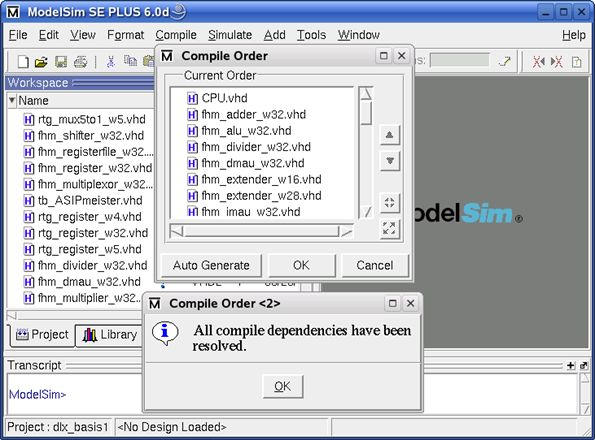
\includegraphics[width=6.19375in,height=4.58194in]{5-3.png}

Figure 5‑3: Compiling the Project

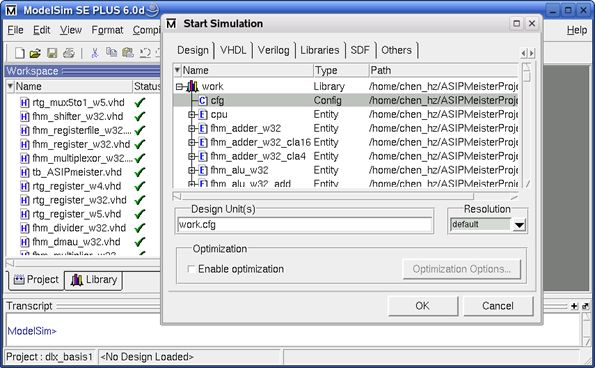
\includegraphics[width=6.19375in,height=3.83611in]{5-4.png}

Figure 5‑4\protect\hypertarget{Fig54}{}{}: Starting the ModelSim
Simulation

Select the \emph{wave\_vhdl.do} file in your \emph{ModelSim} directory
and press OK to load it. The wave-window will be filled with certain
signals that are useful to evaluate the simulation of the program
running on the processor. These signals are explained in Chapter~5.1.5.

Press the button \emph{Run all} to run the simulation until it aborts.
At the end of a simulation the message ``\emph{Failure: Simulation
End}'' is printed. The type ``\emph{Failure}'' is only used to
automatically abort the simulation. This is not a real failure. At the
simulation end, the file \emph{TestData.OUT} is created in your
\emph{ModelSim} directory. It contains the content of the simulated
memory after the CPU finished working. Therefore, if your algorithm is
storing the result in the memory you can find the values here.

If you want to run another simulation with a modified program or with a
modified initial data memory on the same CPU, then execute again
``\emph{make sim}'' in the respective application subdirectory to create
the new \emph{TestData.IM} and \emph{TestData.DM} and afterwards you
have to press the buttons \emph{restart} and \emph{run all}, like shown
in \protect\hyperlink{Fig55}{Figure 5-5}.

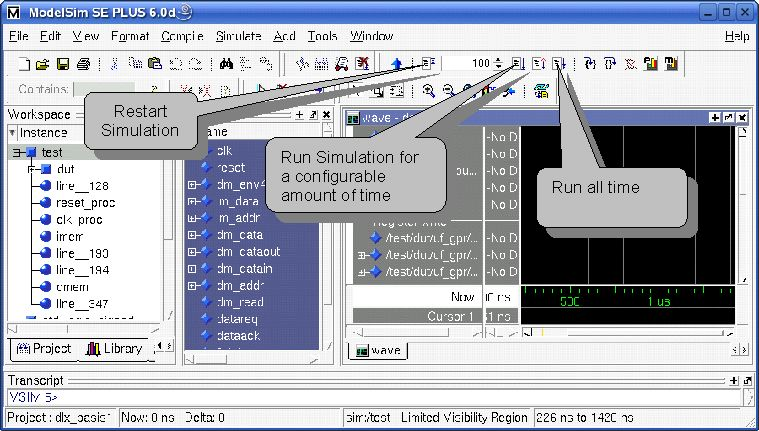
\includegraphics[width=6.29097in,height=3.58125in]{5-5.png}

Figure 5‑5:\protect\hypertarget{Fig55}{}{} Running the ModelSim
Simulation

\hypertarget{statistics-of-the-simulation}{%
\subsubsection{Statistics of the
Simulation}\label{statistics-of-the-simulation}}

During simulation time, the testbench prints status messages about
memory access (Load/Store operations) into the workspace status window.
Thus, you can see which operation is being executed and which values are
being stored and loaded. The following examples show a read and a write
access:

\# ClockCycle:23 InstrAddr:0x00000042 DMemAddr:0x0000FFF0
-\/-\textgreater{} 0 (Read)

\# ClockCycle:30 InstrAddr:0x00000049 DMemAddr:0x0000FFF4 \textless-\/-
0 (Write 32-Bit) (Old value was 45)

The read access is performed in cycle 23 while the currently requested
instruction memory address (\emph{IM\_addr\_out}) is 0x42. This does not
mean, that the corresponding load instruction is fetched into the
pipeline in cycle 23 or that this load instruction is placed at
\emph{IM\_addr\_out} 0x42. Instead, this means that the MEM-Phase of the
corresponding load instruction is executed in cycle 23 and that the
instruction at address 0x42 is fetched into the pipeline, while this
load instruction is performing its MEM phase. The corresponding load
instruction is usually placed some instructions before the printed
\emph{IM\_addr\_out}, unless there was a jump in between. The loaded
value is zero in the printed example and this value comes from address
0xFFF0. This is a stack operation, as the stack is starting at address
0xFFFF and growing downwards in our case (but the starting address of
the stack might be a subject of changes). The loaded value is zero in
this example. The afterwards printed write-example additionally shows
which value is placed in the memory location that is to be overwritten.

A more detailed kind of statistics for the simulation is the wave
diagram as shown in \protect\hyperlink{Fig56}{Figure 5-6}. The waves
show the internal details of the VHDL model that is simulated. The waves
are grouped into five parts, which are explained in Figure 5‑7:. For
more details of the memory signals, see Page-47 in {[}RM{]}.

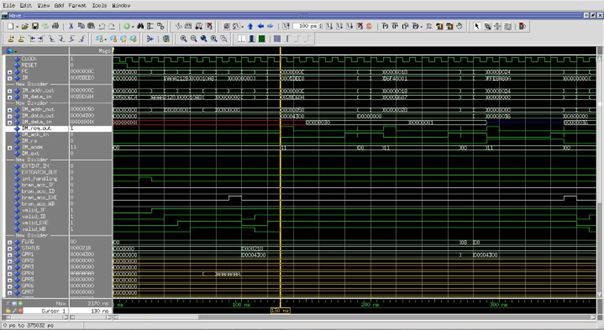
\includegraphics[width=6.29444in,height=3.43611in]{5-7.jpg}

Figure 5‑6:\protect\hypertarget{Fig56}{}{} ModelSim Waveforms

To add additional signal to the Wave window (which is very helpful for
debugging) you need to enable two views in ModelSim (both are enabled by
default):

Menu: View \textgreater{} Workspace

Menu: View \textgreater{} Debug Windows \textgreater{} Objects

\begin{longtable}[]{@{}ll@{}}
\toprule
\textbf{Signal} & \textbf{Explanation}\tabularnewline
\midrule
\endhead
RESET & The \emph{reset} signal of the CPU. This signal is active at the
beginning of every simulation to initialize the CPU.\tabularnewline
CLOCK & The \emph{clock} signal of the CPU. This signal is helpful to
see, when other signal changes are really taken into the CPU, as they
are only sampled at the rising edge of the clock.\tabularnewline
PC & Program counter\tabularnewline
IR & Instruction register\tabularnewline
clock\_counter & The clock counter counts the number of executed clock
cycles since the CPU started running after the initial
reset.\tabularnewline
IM\_addr\_out & This is the Instruction Memory Address. It shows the
address of the instruction that the CPU wants to fetch into its
pipeline.\tabularnewline
IM\_data\_in & This is the Instruction Memory Data that corresponds to
the previous shown \emph{im\_addr}. Therefore, it is the binary
representation of the assembly instruction that is fetched by the
CPU.\tabularnewline
DM\_addr\_out & This is the Address Bus for memory accesses. This bus
either contains the address to which some data will be written or the
address from which some data will be read.\tabularnewline
DM\_data\_out & The Data Bus contains the value that will be written to
the memory.\tabularnewline
DM\_data\_in & The Data Bus contains the value that will be read from
the memory.\tabularnewline
DM\_req\_out & This is the request signal from CPU to trigger a read or
a write access.\tabularnewline
DM\_ack\_in & This is the acknowledge signal, that is activated by the
memory controller after a requested write access is finished or after
the data bus contains the result of a requested read
access.\tabularnewline
DM\_rw & Read from the memory if 0, otherwise write to the
memory.\tabularnewline
DM\_mode & This signal determines the read/write mode. The usual values
are ``11'' for ``word'' and ``00'' for ``byte''
read/write.\tabularnewline
DM\_ext & Sign extension signal\tabularnewline
\begin{minipage}[t]{0.47\columnwidth}\raggedright
EXTINT\_IN

EXTCATCH\_OUT

int\_handling\strut
\end{minipage} & \begin{minipage}[t]{0.47\columnwidth}\raggedright
Interrupt Signals\strut
\end{minipage}\tabularnewline
\begin{minipage}[t]{0.47\columnwidth}\raggedright
bran\_acc\_IF

bran\_acc\_ID

bran\_acc\_EXE

bran\_acc\_WB

valid\_IF

valid\_ID

valid\_EXE

valid\_WB\strut
\end{minipage} & \begin{minipage}[t]{0.47\columnwidth}\raggedright
Pipeline stages information\strut
\end{minipage}\tabularnewline
\begin{minipage}[t]{0.47\columnwidth}\raggedright
FLAG

STATUS

GPR1... GPR31\strut
\end{minipage} & \begin{minipage}[t]{0.47\columnwidth}\raggedright
Register file values\strut
\end{minipage}\tabularnewline
\bottomrule
\end{longtable}

Figure 5‑7: Explanation of the Signals in the ModelSim Waveform

In the ``\emph{Workspace}'', you can choose which instance of your
design will be shown in the ``\emph{Objects}'' windows. From the Objects
window, you can then drag-and-drop signals to the Wave window.

\hypertarget{general-hints}{%
\subsection{General Hints}\label{general-hints}}

\begin{itemize}
\item
  Change to your \emph{ModelSim} directory inside your project directory
  tree and verify that the memory images \emph{TestData.IM} and
  \emph{TestData.DM} are present. The Makefile should have automatically
  created these files. Furthermore, you need the ModelSim testbench file
  \emph{tb\_browstd32.vhd} and the configuration script
  \emph{wave\_vhdl.do}, which are available in the
  \emph{TEMPLATE\_PROJECT/ModelSim} directory. Please make sure that
  these files exist in your \emph{ModelSim} directory before you start
  the simulation. It keeps you safe from trouble.
\item
  Always invoke ModelSim in the specific \emph{ModelSim} directory of
  your current project by executing \emph{vsim \&} in this directory.
  ModelSim is working with project directories and is searching for
  information in the directory where it is invoked. After creating new
  projects all settings will be saved in the project file e.g.
  \emph{projectname.mpf} (where mpf stands for ModelSim Project file).
  To speed up the starting process you can invoke \emph{vsim} with an
  option for your project file that you have created in an earlier
  simulation: ``\emph{vsim projectname.mpf \&''.}
\item
  When you compile VHDL files ModelSim creates a local library in the
  subdirectory \emph{work} to store the compilation results. This is the
  main reason why it is important to start ModelSim in the right place.
  It looks for last project information and for the local library.
\item
  Sometimes you might get compiler errors from the ModelSim VHDL
  compiler. This is usually not the fault of ASIP Meister or the
  testbench. Very often, a ``\emph{recompile all}'' solves this problem.
  However, sometimes you will have to create a new project from the
  scratch to get it working.
\item
  If you open the waves before the simulation is started, then the
  signals will not be displayed. First start the simulation, and then
  open the waves.
\end{itemize}

\end{document}
